\documentclass{oblivoir}
%%%Default packages
\usepackage{amsmath,amssymb,amsthm,kotex,tabu,graphicx,pifont}
\usepackage{../kswrapfig}

\usepackage{gensymb} %\degree

%%%More packages
%\usepackage{caption,subcaption}
%\usepackage[perpage]{footmisc}
%
\usepackage[skipabove=10pt,innertopmargin=10pt,nobreak=true]{mdframed}

\usepackage[inline]{enumitem}
\setlist[enumerate,1]{label=(\arabic*)}
\setlist[enumerate,2]{label=(\alph*)}

\usepackage{multicol}
\setlength{\columnsep}{30pt}
\setlength{\columnseprule}{1pt}
%
%\usepackage{forest}
%\usetikzlibrary{shapes.geometric,arrows.meta,calc}
%
%%%defi theo exam prob rema proo
%이 환경들 아래에 문단을 쓸 경우 살짝 들여쓰기가 되므로 \hspace{-.7em}가 필요할 수 있다.

\newcounter{num}
\newcommand{\defi}[1]
{\noindent\refstepcounter{num}\textbf{정의 \arabic{num})} #1\par\noindent}
\newcommand{\theo}[1]
{\noindent\refstepcounter{num}\textbf{정리 \arabic{num})} #1\par\noindent}
\newcommand{\revi}[1]
{\noindent\refstepcounter{num}\textbf{복습 \arabic{num})} #1\par\noindent}
\newcommand{\exam}[1]
{\bigskip\bigskip\noindent\refstepcounter{num}\textbf{예시 \arabic{num})} #1\par\noindent}
\newcommand{\prob}[1]
{\bigskip\bigskip\noindent\refstepcounter{num}\textbf{문제 \arabic{num})} #1\par\noindent}
\newcommand{\rema}[1]
{\bigskip\bigskip\noindent\refstepcounter{num}\textbf{참고 \arabic{num})} #1\par\noindent}
\newcommand{\proo}
{\bigskip\noindent\textsf{증명)}}

\newenvironment{talign}
 {\let\displaystyle\textstyle\align}
 {\endalign}
\newenvironment{talign*}
 {\let\displaystyle\textstyle\csname align*\endcsname}
 {\endalign}
%
%%%Commands

\newcommand{\procedure}[1]{\begin{mdframed}\vspace{#1\textheight}\end{mdframed}}

\newcommand\an[1]{\par\bigskip\noindent\textbf{문제 \ref{#1})}\par\noindent}

\newcommand\ann[2]{\par\bigskip\noindent\textbf{문제 \ref{#1})}\:\:#2\par\medskip\noindent}

\newcommand\ans[1]{\begin{flushright}\textbf{답 : }#1\end{flushright}}

\newcommand\anssec[1]{\bigskip\bigskip\noindent{\large\bfseries#1}}

\newcommand{\pb}[1]%\Phantom + fBox
{\fbox{\phantom{\ensuremath{#1}}}}

\newcommand\ba{\,|\,}

\newcommand\ovv[1]{\ensuremath{\overline{#1}}}
\newcommand\ov[2]{\ensuremath{\overline{#1#2}}}
%
%%%% Settings
%\let\oldsection\section
%
%\renewcommand\section{\clearpage\oldsection}
%
%\let\emph\textsf
%
%\renewcommand{\arraystretch}{1.5}
%
%%%% Footnotes
%\makeatletter
%\def\@fnsymbol#1{\ensuremath{\ifcase#1\or
%*\or **\or ***\or
%\star\or\star\star\or\star\star\star\or
%\dagger\or\dagger\dagger\or\dagger\dagger\dagger
%\else\@ctrerr\fi}}
%
%\renewcommand{\thefootnote}{\fnsymbol{footnote}}
%\makeatother
%
%\makeatletter
%\AtBeginEnvironment{mdframed}{%
%\def\@fnsymbol#1{\ensuremath{\ifcase#1\or
%*\or **\or ***\or
%\star\or\star\star\or\star\star\star\or
%\dagger\or\dagger\dagger\or\dagger\dagger\dagger
%\else\@ctrerr\fi}}%
%}   
%\renewcommand\thempfootnote{\fnsymbol{mpfootnote}}
%\makeatother
%
%%% 객관식 선지
\newcommand\one{\ding{172}}
\newcommand\two{\ding{173}}
\newcommand\three{\ding{174}}
\newcommand\four{\ding{175}}
\newcommand\five{\ding{176}}
\usepackage{tabto,pifont}
%\TabPositions{0.2\textwidth,0.4\textwidth,0.6\textwidth,0.8\textwidth}

\newcommand\taba[5]{\par\noindent
\one\:{#1}
\tabto{0.2\textwidth}\two\:\:{#2}
\tabto{0.4\textwidth}\three\:\:{#3}
\tabto{0.6\textwidth}\four\:\:{#4}
\tabto{0.8\textwidth}\five\:\:{#5}}

\newcommand\tabb[5]{\par\noindent
\one\:{#1}
\tabto{0.33\textwidth}\two\:\:{#2}
\tabto{0.67\textwidth}\three\:\:{#3}\medskip\par\noindent
\four\:\:{#4}
\tabto{0.33\textwidth}\five\:\:{#5}}

\newcommand\tabc[5]{\par\noindent
\one\:{#1}
\tabto{0.5\textwidth}\two\:\:{#2}\medskip\par\noindent
\three\:\:{#3}
\tabto{0.5\textwidth}\four\:\:{#4}\medskip\par\noindent
\five\:\:{#5}}

\newcommand\tabd[5]{\par\noindent
\one\:{#1}\medskip\par\noindent
\two\:\:{#2}\medskip\par\noindent
\three\:\:{#3}\medskip\par\noindent
\four\:\:{#4}\medskip\par\noindent
\five\:\:{#5}}
%
%%%% fonts
%
%\usepackage{fontspec, xunicode, xltxtra}
%\setmainfont[]{은 바탕}
%\setsansfont[]{은 돋움}
%\setmonofont[]{은 바탕}
%\XeTeXlinebreaklocale "ko"
%%%%
\begin{document}

\title{수학Ⅰ : 01 지수}
\author{}
\date{\today}
\maketitle
\tableofcontents
\newpage

%%%
\section{복습}

%
\prob{다음 식을 전개하시오.}
\begin{enumerate}[itemsep=10pt]\label{review1}
\item
\((a+b)(a-b)\)
\item
\((a+bi)(a-bi)\)
\item
\((a-b)(a^2+ab+b^2)\)
\end{enumerate}

%
\prob{다음 식을 인수분해하시오.}
\begin{enumerate}[itemsep=10pt]\label{review2}
\item
\(a^3+b^3\)
\item
\(x^3-27\)
\item
\(x^2-1\)
\item
\(x^2-5\)
\item
\(x^2+9\)
\item
\(x^4-16\)
\end{enumerate}

\begin{mdframed}[frametitle={기본적인 인수분해 공식}]
\begin{enumerate}
\item
\(a^2-b^2=(a+b)(a-b)\)
\item
\(a^3+b^3=(a+b)(a^2-ab+b^2)\)
\item
\(a^3-b^3=(a-b)(a^2+ab+b^2)\)
\end{enumerate}
\end{mdframed}
\newpage

%
\prob{다음 이차방정식을 푸시오.}\label{review3}
\par\noindent
(1)\:\:\(x^2=4\)
\tabto{.333\textwidth}
(2)\:\:\(x^2=0\)
\tabto{.666\textwidth}
(3)\:\:\(x^2=-4\)
\par\noindent
(4)\:\:\(x^2-x-2=0\)
\tabto{.333\textwidth}
(5)\:\:\(x^2-x-1=0\)
\tabto{.666\textwidth}
(6)\:\:\(x^2+2x+2=0\)
\begin{mdframed}
\vspace{0.3\textheight}
\end{mdframed}
{\par\raggedleft\textbf{답 :
(1)\:\:\(x=\)\qquad\qquad(2)\:\:\(x=\)\qquad\qquad(3)\:\:\(x=\)\qquad\qquad\qquad}
\par}
{\par\raggedleft\textbf{
(4)\:\:\(x=\)\qquad\qquad(5)\:\:\(x=\)\qquad\qquad(6)\:\:\(x=\)\qquad\qquad\qquad}
\par}
\bigskip

\begin{mdframed}[frametitle={이차방정식의 풀이}]
\begin{enumerate}\label{review4}
\item
이차방정식 \(x^2=A\)의 근은
\[x=\pm\sqrt A\]
\item
이차방정식 \(ax^2+bx+c=0\)의 근은
\[x=\frac{-b\pm\sqrt{b^2-4ac}}{2a}\]
\item
\(b\)가 짝수이면 (\(b=2b'\))
\[x=\frac{-b'\pm\sqrt{b'^2-ac}}a\]
\end{enumerate}
\end{mdframed}

%
\section{제곱근}
%
\begin{mdframed}
\defi{\(a\)의 제곱근}\label{sqroot1}
제곱해서 \(a\)가 되는 수를 \(A\)의 \fbox{제곱근}이라고 한다.
\end{mdframed}

%
\exam{9의 제곱근을 구하여라.}\label{sqroot2}
\vspace{-10pt}
\begin{mdframed}
\(x^2=9\)
를 만족시키는 수 \(x\)를 구하면 된다.
\begin{gather*}
x^2-9		=0\\
(x+3)(x-3)	=0
\end{gather*}
이므로 \(x=3\) 또는 \(x=-3\) 이다.
\end{mdframed}
\ans{\(3,\;-3\)}

%
\exam{\(-9\)의 제곱근을 구하여라.}\label{sqroot3}
\vspace{-10pt}
\begin{mdframed}
\(x^2=-9\)
를 만족시키는 수 \(x\)를 구하면 된다.
\begin{gather*}
x^2+9		=0\\
(x+3i)(x-3i)	=0
\end{gather*}
이므로 \(x=3i\) 또는 \(x=-3i\) 이다.
\end{mdframed}
\ans{\(3i,\;-3i\)}

%
\prob{다음 수들의 제곱근을 각각 구하여라.}\label{sqroot4}
\\[-10pt]
\begin{enumerate*}[itemjoin=\hspace{0.25\textwidth}]
\item
4
\item
0
\item
\(-25\)
\end{enumerate*}

\newpage
%
\begin{mdframed}
\defi{\(\sqrt a\)}\label{sqroot5}
\(a\)가 \fbox{양수}일 때, \(a\)의 제곱근 중 \fbox{양수}인 것을 `제곱근 \(a\)' 또는 \(\sqrt a\)라고 한다.
\end{mdframed}

%
\exam{}\label{sqroot6}
예시 \ref{sqroot2})에서 9의 제곱근 중 양수인 것은 \(3\)이므로 제곱근 9는 3이다.
즉
\[\sqrt9=3\]
이다.

%%
%\rema{\(a\le0\)일 때,}
%\begin{enumerate}
%\item
%\(\sqrt{-9}=\sqrt3i\)
%\item
%\(\sqrt0=0\)
%\end{enumerate}

%
\prob{다음을 간단히 하여라.}
\begin{enumerate}\label{sqroot7}
\item
\(\sqrt{16}\)
\item
\(\sqrt{36}\)
%\item
%\(\sqrt{-25}\)
\end{enumerate}

%
\begin{mdframed}
\defi{제곱근의 성질}\label{sqroot8}
\(a>0\), \(b>0\)일 때,
\begin{enumerate}
%\item
%\(a>0\)일 때, \((\sqrt a)^2=a\)
%\item
%\(a\)가 실수일 때, \(\sqrt{a^2}=|a|\)
\item
\(\sqrt{ab}=\sqrt a\sqrt b\)
\item
\(\sqrt{\frac ab}=\frac{\sqrt a}{\sqrt b}\)
\end{enumerate}
\end{mdframed}

%
\exam{\(\sqrt{12}\)를 간단히 하여라.}\label{sqroot9}
\\
\(\sqrt{12}=\sqrt{4\cdot3}\stackrel{(1)}=\sqrt4\sqrt3=2\sqrt3\)

%
\prob{다음을 간단히 하여라.}
\begin{enumerate}\label{sqroot10}
\item
\(\sqrt{54}\)
\item
\(\sqrt{80}\)
\item
\(\sqrt{\frac23}\)
\end{enumerate}

%%
\section{거듭제곱근}
%
\begin{mdframed}
\defi{\(a\)의 세제곱근}\label{nthroot1}
세제곱해서 \(a\)가 되는 수를 \(a\)의 \fbox{세제곱근}이라고 한다.
\end{mdframed}

%
\exam{27의 세제곱근을 구하여라.}\label{nthroot2}
\vspace{-10pt}
\begin{mdframed}
\(x^3=27\)
를 만족시키는 수 \(x\)를 구하면 된다.
\begin{gather*}
x^3-27			=0\\
(x-3)(x^2+3x+9)	=0
\end{gather*}
이므로 \(x=3\) 또는 \(x^2+3x+9=0\) 이다.
즉
\(x=3\) 또는 \(x=\frac{-3\pm3\sqrt3i}2\)이다.
\end{mdframed}
\ans{\(3\),\;\(\frac{-3+3\sqrt3i}2\),\;\(\frac{-3-3\sqrt3i}2\)}

%
\exam{\(-27\)의 세제곱근을 구하여라.}\label{nthroot3}
\vspace{-10pt}
\begin{mdframed}
\(x^3=-27\)
를 만족시키는 수 \(x\)를 구하면 된다.
\begin{gather*}
x^3+27			=0\\
(x+3)(x^2-3x+9)	=0
\end{gather*}
이므로 \(x=-3\) 또는 \(x^2-3x+9=0\) 이다.
즉
\(x=-3\) 또는 \(x=\frac{3\pm3\sqrt3i}2\)이다.
\end{mdframed}
\ans{\(-3\),\;\(\frac{3+3\sqrt3i}2\),\;\(\frac{3-3\sqrt3i}2\)}

%
\prob{다음 수들의 세제곱근을 각각 구하여라.}\label{nthroot4}
\\
\begin{enumerate*}[itemjoin=\hspace{0.2\textwidth}]
\item
8
\item
\(-8\)
\item
\(1\)
\item
\(-1\)
\end{enumerate*}

\newpage
%
\begin{mdframed}
\defi{\(\sqrt[3]a\)}\label{nthroot5}
\(a\)가 \fbox{실수}일 때, \(a\)의 세제곱근 중 \fbox{실수}인 것을 `세제곱근 \(a\)' 또는 \(\sqrt[3]a\)라고 한다.
\end{mdframed}

%
\exam{}
\begin{enumerate}\label{nthroot6}
\item
예시 \ref{nthroot2})에서 27의 세제곱근 중 실수인 것은 \(3\)이므로 세제곱근 27는 3이다.
즉
\[\sqrt[3]{27}=3\]
이다.
\item
예시 \ref{nthroot3})에서 \(-27\)의 세제곱근 중 실수인 것은 \(-3\)이므로 세제곱근 \(-27\)는 \(-3\)이다.
즉
\[\sqrt[3]{-27}=-3\]
이다.
\end{enumerate}

%
\prob{다음을 간단히 하여라.}
\begin{enumerate}\label{nthroot7}
\item
\(\sqrt[3]8\)
\item
\(\sqrt[3]{-8}\)
\item
\(\sqrt[3]1\)
\item
\(\sqrt[3]{-1}\)
\end{enumerate}

\newpage
%
\exam{81의 네제곱근을 구하여라.}\label{nthroot8}
\vspace{-10pt}
\begin{mdframed}
\(x^4=81\)
를 만족시키는 수 \(x\)를 구하면 된다.
\begin{gather*}
x^4-81				=0\\
(x^2-9)(x^2+9)			=0\\
(x+3)(x-3)(x+3i)(x-3i)	=0
\end{gather*}
이므로 \(x=\pm3\), \(x=\pm3i\) 이다.
\end{mdframed}
\ans{\(3\), \(-3\), \(3i\), \(-3i\)}

%
\prob{다음 수들의 네제곱근을 각각 구하여라.}\label{nthroot9}
\\[-10pt]
\begin{enumerate*}[itemjoin=\hspace{0.25\textwidth}]
\item
0
\item
16
\item
4
\end{enumerate*}

\bigskip

%
\begin{mdframed}
\defi{\(\sqrt[4]a\)}\label{nthroot10}
\(a\)가 \fbox{양수}일 때, \(a\)의 네제곱근 중 \fbox{양수}인 것을 `네제곱근 \(a\)' 또는 \(\sqrt[4]a\)라고 한다.
\end{mdframed}

%
\exam{}\label{nthroot11}
예시 \ref{nthroot8})에서 81의 네제곱근 중 양수인 것은 \(3\)이므로 네제곱근 81은 3이다.
따라서
\[\sqrt[4]{81}=3\]
이다.

%
\prob{다음을 간단히 하여라.}
\begin{enumerate}\label{nthroot12}
\item
\(\sqrt[4]{16}\)
\item
\(\sqrt[4]{4}\)
\end{enumerate}

\newpage
정리 \ref{sqroot5}), \ref{nthroot5}), \ref{nthroot10})을 잘 살펴보면, \(n\)제곱근 \(a\)는 \(n\)이 짝수인지 홀수인지에 따라 정의가 달라진다는 것을 볼 수 있다.

%
\begin{mdframed}
\defi{\(\sqrt[n]a\)}
\begin{enumerate}[label=\roman*)]\label{nthroot13}
\item
\(n\)이 짝수이면, \(a\)가 \fbox{양수}일 때
\[\sqrt[n]a=\text{\(a\)의 \(n\)제곱근 중 \fbox{양수}인 것}\]
%\(a\)의 \(n\)제곱근 중 \fbox{양수}인 것을 \(n\)제곱근 \(a\) 또는 \(\sqrt[n]a\)라고 한다.
\item
\(n\)이 홀수이면, \(a\)가 \fbox{실수}일 때
\[\sqrt[n]a=\text{\(a\)의 \(n\)제곱근 중 \fbox{실수}인 것}\]
%\(a\)의 \(n\)제곱근 중 \fbox{실수}인 것을 \(n\)제곱근 \(a\) 또는 \(\sqrt[n]a\)라고 한다.
\end{enumerate}
\end{mdframed}
만약 \(n=2\)이면 \(\sqrt[2]a\)의 \(2\)를 생략해 \(\sqrt a\)로 쓴다.

%
\exam{}
\begin{enumerate}\label{nthroot14}
\item
\(\sqrt{64}=\text{64의 제곱근 중에 \fbox{양수}인 것}=8\)
\item
\(\sqrt{-64}\quad\Longrightarrow\)\quad\(-64\)가 음수이므로 \(\sqrt{-64}\)는 생각하지 않는다.\footnotemark
\item
\(\sqrt[3]{64}=\text{64의 세제곱근 중에 \fbox{실수}인 것}=4\)
\item
\(\sqrt[3]{-64}=\text{\(-64\)의 세제곱근 중에 \fbox{실수}인 것}=-4\)
\item
\(\sqrt[4]{64}=\text{64의 네제곱근 중에 \fbox{양수}인 것}=2\sqrt2\)
\item
\(\sqrt[4]{-64}\quad\Longrightarrow\)\quad\(-64\)가 음수이므로 \(\sqrt{-64}\)는 생각하지 않는다.
\end{enumerate}
\footnotetext{굳이 \(\sqrt{-64}\)를 구하면
\[\sqrt{-64}=\sqrt{64}i=8i\]
가 되어 허수가 나온다.}

\newpage
%
\rema{}
\begin{enumerate}\label{nthroot15}
\begin{minipage}{0.6\textwidth}
\item
\(n\)이 짝수이면,  함수 \(y=x^n\)의 그래프는\\
\(y\)축에 대해서 대칭인 그래프이다(우함수).\\
따라서 \(a\)가 양수이면 \(y=x^n\)의 그래프와\\
\(y=a\)의 그래프의 교점은 두 개이며, 그중\\
\(x\)가 양수인 것은 단 하나 존재한다.
\end{minipage}
\begin{minipage}{.3\textwidth}
\begin{center}
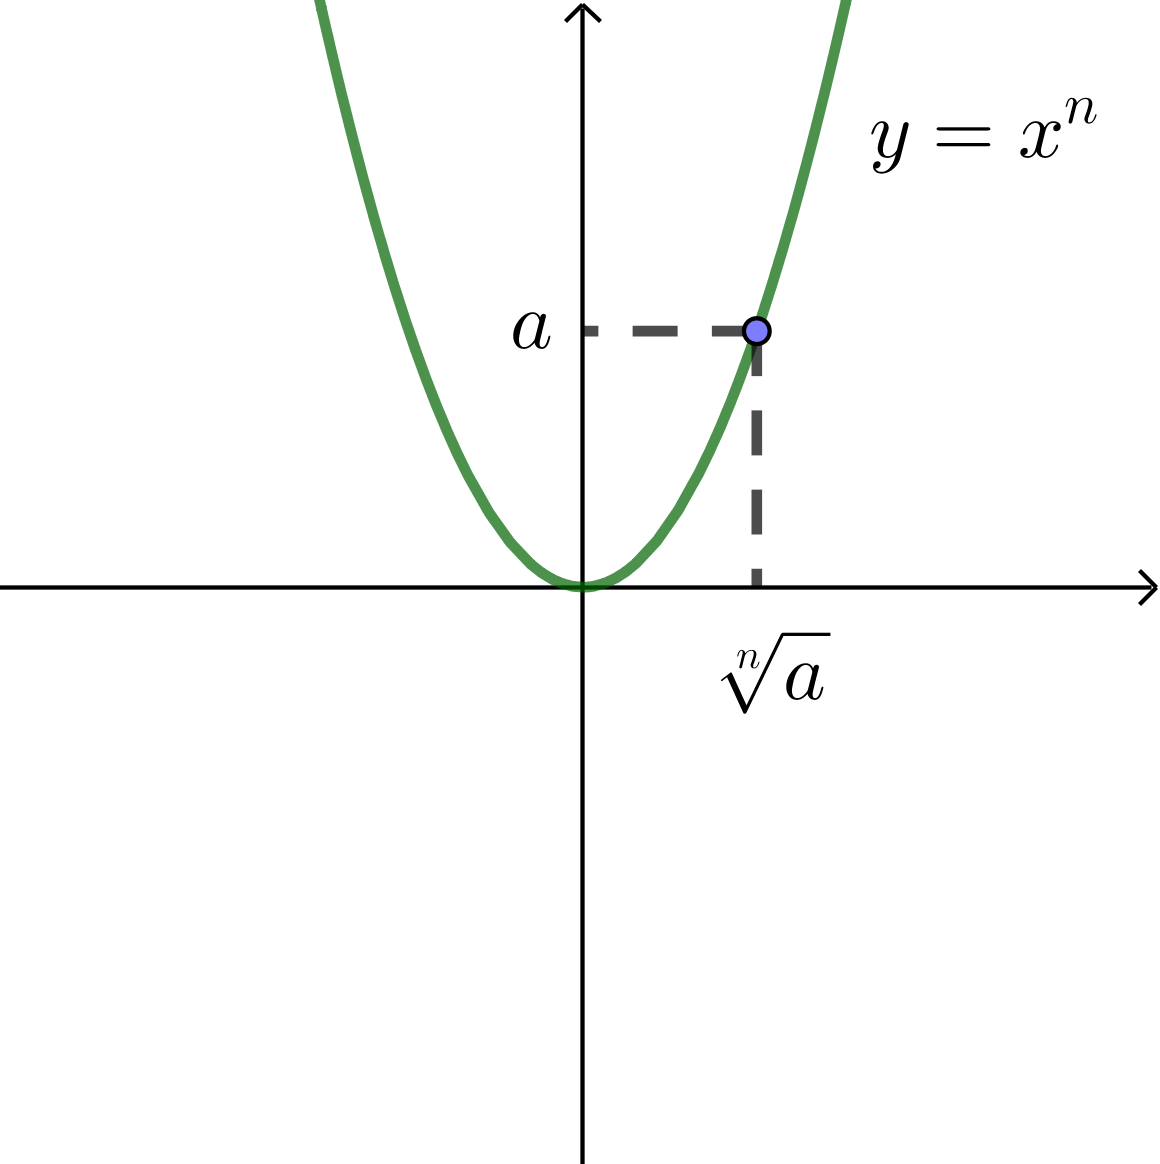
\includegraphics[height=0.2\textheight]{nthroot-even}
\end{center}
\end{minipage}
\par
즉, \(a\)가 \fbox{양수}이면, \(x^n=a\)를 만족시키는  \fbox{양수} \(x\)는 단 하나 존재한다.
\begin{minipage}{0.6\textwidth}\
\item
\(n\)이 홀수이면,  함수 \(y=x^n\)의 그래프는\\
원점에 대해서 대칭인 그래프이다(기함수).\\
따라서 \(a\)가 양수이건 음수이건 상관없이\\
\(y=x^n\)의 그래프와 \(y=a\)의 그래프의 교점은 한 개이다.
\end{minipage}
\begin{minipage}{.3\textwidth}
\begin{center}
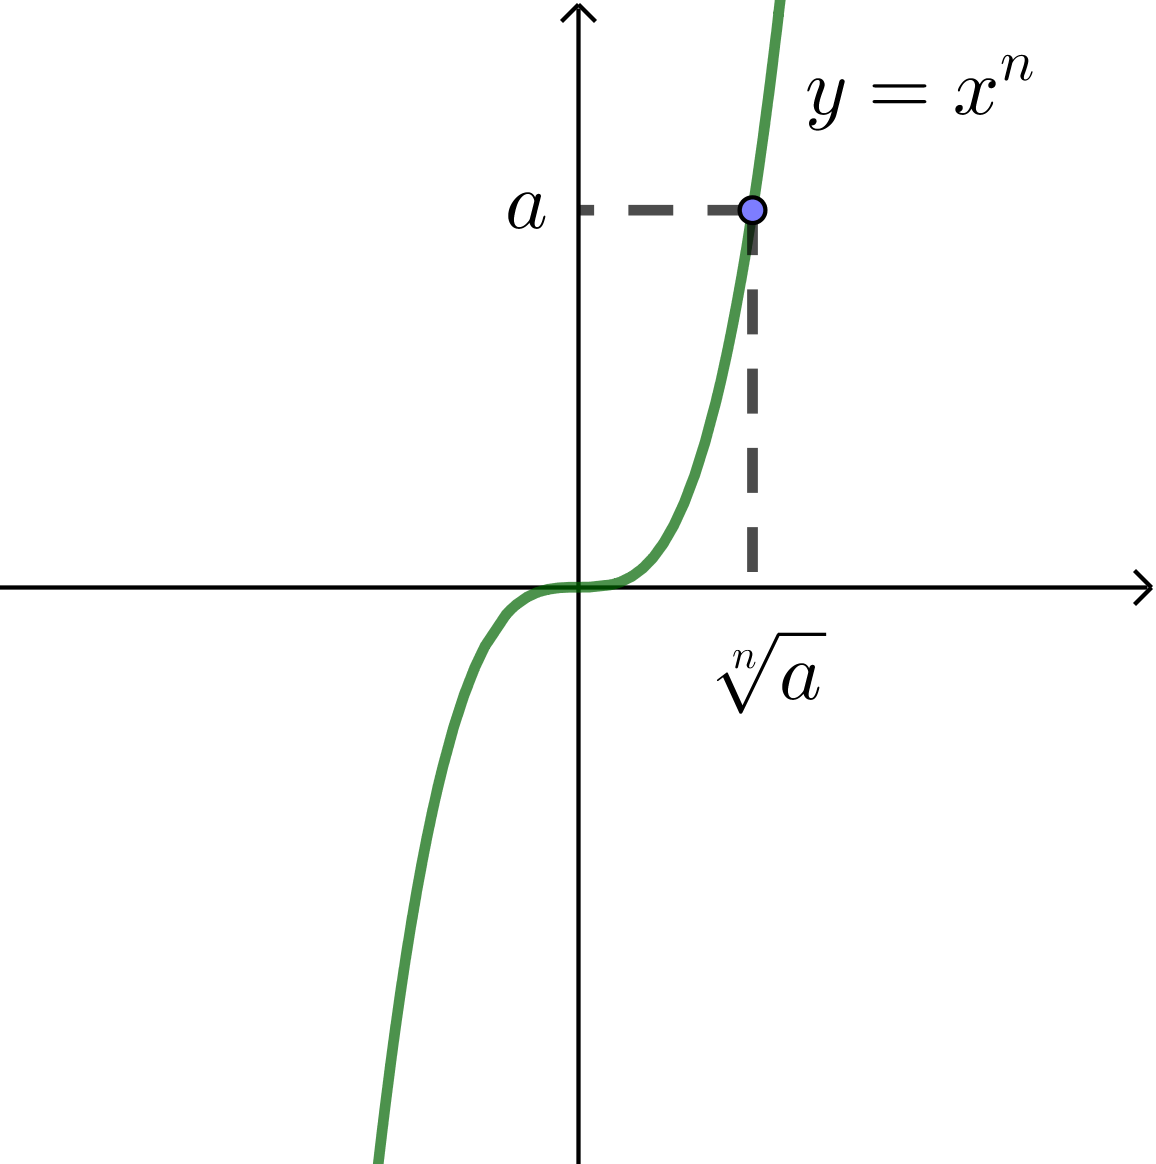
\includegraphics[height=0.2\textheight]{nthroot-odd}
\end{center}
\end{minipage}
\par
즉, \(a\)가 \fbox{실수}이면, \(x^n=a\)를 만족시키는  \fbox{실수} \(x\)는 단 하나 존재한다.
\end{enumerate}

%%
%\prob{다음 중 옳지 않은 것을 고르시오.}\label{nthroot16}
%\tabd
%{125의 세제곱근은 세 개이다.}
%{125의 세제곱근 중 실수인 것은 한 개이다.}
%{\(\sqrt[3]{125}\)는 양수이다.}
%{\(-4\)의 제곱근은 두 개이다.}
%{\(-4\)의 제곱근 중 실수인 것은 두 개이다.}
%
%%
%\prob{다음 중 옳지 않은 것을 고르시오.}\label{nthroot17}
%\tabc
%{\(\sqrt[3]5>0\)}
%{\(\sqrt[3]{-5}<0\)}
%{\(\sqrt[4]5>0\)}
%{\(\sqrt[4]{-5}<0\)}
%{\(\sqrt[5]5>0\)}

%
\exam{다음 값을 구하여라.}\label{nthroot18}
\par\noindent
(1)\:\:\(\sqrt[3]{-27}\)
\tabto{.25\textwidth}
(2)\:\:\(\sqrt[5]{100000}\)
\tabto{.5\textwidth}
(3)\:\:\(\sqrt[4]{\frac{16}{81}}\)
\tabto{.75\textwidth}
(4)\:\:\(-\sqrt[4]{0.0625}\)
\begin{mdframed}
\begin{enumerate}
\item
\((-3)^3=-27\)이므로 \(\sqrt[3]{-27}=-3\)이다.
\item
\(10^5=100000\)이므로 \(\sqrt[5]{100000}=10\)이다.
\item
\(\left(\frac23\right)^4=\frac{16}{81}\)이므로 \(\sqrt[4]{\frac{16}{81}}=\frac23\)이다.
\item
\(0.5^4=0.0625\)이므로 \(\sqrt[4]{0.0625}=0.5\)이다.
따라서 \(-\sqrt[4]{0.0625}=-0.5\)
\end{enumerate}
\end{mdframed}
{\par\raggedleft\textbf{답 :
(1)\:\:\(-3\)\quad(2)\:\:\(10\)\:\:(3)\:\:\(\frac23\)\quad(4)\:\:\(-0.5\)}\par}\bigskip

%
\prob{다음 값을 구하여라.}\label{nthroot19}
\par\noindent
(1)\:\:\(\sqrt[5]{32}\)
\tabto{.25\textwidth}
(2)\:\:\(-\sqrt[4]{0.0016}\)
\tabto{.5\textwidth}
(3)\:\:\(-\sqrt[3]{-0.125}\)
\tabto{.75\textwidth}
(4)\:\:\(\sqrt[4]{\frac1{256}}\)

%%
\section{거듭제곱근의 성질}
%
\exam{\(\sqrt[3]8\times\sqrt[3]{27}\)과 \(\sqrt[3]{8\times27}\) 을 각각 계산해보면}\label{property1}
\vspace{-20pt}
\begin{align*}
\sqrt[3]8\times\sqrt[3]{27}&=2\times3=6\\
\sqrt[3]{8\times27}&=\sqrt[3]{216}=6
\end{align*}
이다.
따라서
\vspace{-5pt}
\[\sqrt[3]8\times\sqrt[3]{27}=\sqrt[3]{8\times27}\]
이다.
\(a>0\), \(b>0\)에 대하여
\vspace{-5pt}
\[\sqrt a\sqrt b=\sqrt{ab}\]
가 성립하듯
\vspace{-5pt}
\[\sqrt[n]a\sqrt[n]b=\sqrt[n]{ab}\]
도 성립할 것이다.

%
\begin{mdframed}
\theo{\normalfont{\(a>0\), \(b>0\)이고 \(m\), \(n\)이 2이상의 정수일 때,}}
\begin{enumerate}[label=(\alph*)]\label{property2}
\item
\(\displaystyle\sqrt[n]a\sqrt[n]b=\sqrt[n]{ab}\)
\item
\(\displaystyle\frac{\sqrt[n]a}{\sqrt[n]b}=\sqrt[n]{\frac ab}\)
\item
\(\displaystyle(\sqrt[n]a)^m=\sqrt[n]{a^m}\)
\item
\(\displaystyle\sqrt[m]{\sqrt[n]a}=\sqrt[mn]{a}\)
\end{enumerate}
\end{mdframed}

%
\exam{(a)를 증명하여라.}\label{property3}
좌변을 \(n\)제곱하면
\[\big(\sqrt[n]a\sqrt[n]b\big)^n=\big(\sqrt[n]a\big)^n\big(\sqrt[n]b\big)^n=ab\]
이다.
이때, \(\sqrt[n]a\sqrt[n]b>0\)이므로
\(\sqrt[n]a\sqrt[n]b\)는 \(ab\)의 양의 \(n\)제곱근인 \(\sqrt[n]{ab}\)와 같다.
따라서 (a)가 성립한다.

%
\prob{다음은 (b), (c), (d)를 증명하는 과정이다.
빈칸에 알맞은 것을 써넣어라.}\label{property4}
\begin{mdframed}
\begin{enumerate}
\item[(b)]
좌변을 \(n\)제곱하면
\[\Big(\frac{\sqrt[n]a}{\sqrt[n]b}\Big)^n=\frac{\big(\pb{\sqrt[n]a}\big)^n}{\big(\pb{\sqrt[n]b}\big)^n}=\pb{\frac ab}\]
이때, \(\frac{\sqrt[n]a}{\sqrt[n]b}>0\)이므로
\(\frac{\sqrt[n]a}{\sqrt[n]b}\)는 \(\pb{\frac ab}\)의 양의 \(n\)제곱근인 \(\sqrt[n]{\pb{\frac ab}}\)와 같다.
따라서 (b)가 성립한다.
\item[(c)]
좌변을 \(n\)제곱하면
\[\{(\sqrt[n]a)^m\}^n=(\sqrt[n]a)^{mn}=\{(\sqrt[n]a)^n\}^m=\pb{a^m}\]
이때, \((\sqrt[n]a)^m>0\)이므로 \((\sqrt[n]a)^m\)은 \(\pb{a^m}\)의 양의 \(n\)제곱근인 \(\sqrt[n]{\pb{a^m}}\)과 같다.
따라서 (c)가 성립한다.
\item[(d)]
좌변을 \(mn\)제곱하면
\[\left(\sqrt[m]{\sqrt[n]a}\right)^{mn}
=\left\{\left(\sqrt[m]{\sqrt[n]a}\right)^m\right\}^n
=\big(\pb{\sqrt[n]a}\big)^n
=\pb a
\]
이때, \(\sqrt[m]{\sqrt[n]a}>0\)이므로 \(\sqrt[m]{\sqrt[n]a}\)는 \(\pb a\)의 양의 \(mn\)제곱근인 \(\sqrt[mn]{\pb a}\)와 같다.
따라서 (d)가 성립한다.
\end{enumerate}
\end{mdframed}

%
\prob{다음 식을 간단히 하시오.}
\begin{enumerate}\label{property5}
\item
\(\sqrt[3]4\times\sqrt[3]2\)
\item
\(\displaystyle\frac{\sqrt[3]{54}}{\sqrt[3]2}\)
\item
\(\left(\sqrt[3]3\right)^6\)
\item
\(\sqrt[3]{\sqrt[4]{5^{24}}}\)
\end{enumerate}

%%
\section{자연수 지수}
\(a^x\)
와 같이 생긴 것을 \fbox{거듭제곱}이라고 부른다.
이때 \(a\)를 \fbox{밑}, \(x\)를 \fbox{지수}라고 부른다.

%
\prob{다음을 계산하여라.}\label{natural1}
\\[-10pt]
\begin{enumerate*}[itemjoin=\hspace{0.25\textwidth}]
\item
\(5^2\)
\item
\(3^4\)
\item
\(2^7\)
\end{enumerate*}

\begin{mdframed}
%
\defi{자연수 지수}\label{natural2}
\(a\)가 실수이고 \(n\)이 자연수일 때,
\[a^n=\underbrace{a\times a\times\cdots\times a}_\text{$n$ 개}\]
\end{mdframed}

%
\prob{다음 \(\square\)에 알맞은 수를 써넣으시오.}\label{natural3}
\\[-10pt]
\begin{enumerate*}[itemjoin=\hspace{0.15\textwidth}]
\item
\(5^3\times5^4=5^\square\)
\item
\(8^2\times4^2=2^\square\)
\item
\(6^5\div6^2=6^\square\)
\end{enumerate*}

\bigskip\noindent
자연수 지수에 대해 다음 성질들이 성립한다.
%
\begin{mdframed}
\theo{지수법칙 - 자연수 지수}\label{natural4}
\(a\), \(b\)가 실수이고 \(m\), \(n\)이 자연수일 때,
\begin{enumerate}
\item
\(a^m\times a^n=a^{m+n}\)
\item
\(\displaystyle a^m\div a^n=
\begin{cases}
\quad	a^{m-n}		&(m>n)\\
\quad	1			&(m=n)\\
\quad	\frac1{a^{n-m}}&(m<n)
\end{cases}
\)
\item
\((a^m)^n=a^{mn}\)
\item
\((ab)^m=a^mb^m\)
\end{enumerate}
\end{mdframed}

%%
\section{정수 지수}
%
\exam{다음 \(\square\)에 들어갈 수를 유추해보자.}\label{integer1}
\vspace{-20pt}
\begin{gather*}
%2^4		=16\\
2^3		=8\\
2^2		=4\\
2^1		=2\\
2^0		=\pb{0}\\
2^{-1}	=\pb{\frac12}\\
2^{-2}	=\pb{\frac14}
\end{gather*}

\noindent
지수가 정수일 때, 거듭제곱을 다음과 같이 정의한다.
%
\begin{mdframed}
\defi{정수 지수}\label{integer2}
\(a\neq0\)이고 \(n\)이 자연수이면
\begin{enumerate}
\item
\(a^0=1\)
\item
\(\displaystyle a^{-n}=\frac1{a^n}\)
\end{enumerate}
\end{mdframed}
이때, \(0^0\), \(0^{-1}\), \(0^{-2}\) 등은 정의하지 않는다.

%
\exam{}
\begin{enumerate}\label{integer3}
\item
\(2^0=1\)
\item
\((-3)^0=1\)
\item
\(\displaystyle3^{-3}=\frac1{3^3}=\frac1{27}\)
\end{enumerate}

%
\prob{다음 값을 구하여라.}\label{integer4}
\\
\begin{enumerate*}[itemjoin=\hspace{0.15\textwidth}]
\item
\((\sqrt3)^0\)
\item
\(4^{-3}\)
\item
\((-2)^{-3}\)
\item
\(\displaystyle\left(\frac12\right)^{-4}\)
\end{enumerate*}

\newpage
%
\prob{다음 \(\square\)에 알맞은 수를 써넣으시오.}
\begin{enumerate}\label{integer5}
\item
\(3^2\times3^{-3}=3^\square\)
\item
\(5^3\div5^5=5^\square\)
\item
\(\left(2^{-2}\right)^{-3}=2^\square\)
\item
\(15^{-1}=3^\square\times5^\square\)
\end{enumerate}

\noindent
따라서 정수 지수에 대해 다음 성질들이 성립한다.
%
\begin{mdframed}
\theo{지수법칙 - 정수 지수}\label{integer6}
\(a\neq0\), \(b\neq0\)이고 \(m\), \(n\)이 정수일 때,
\begin{enumerate}
\item
\(a^m\times a^n=a^{m+n}\)
\item
\(a^m\div a^n=a^{m-n}\)
\item
\((a^m)^n=a^{mn}\)
\item
\((ab)^m=a^mb^m\)
\end{enumerate}
\end{mdframed}

%
\prob{다음 식을 간단히 하시오.(단, \(a\neq0\), \(b\neq0\))}
\begin{enumerate}\label{integer7}
\item
\(2^4\times3^{-2}\div6^{-3}\)
\item
\((3^3\times9^{-2})^{-1}\)
\item
\(a^3\div(a^2)^{-1}\)
\item
\((a^3b^{-2})^{-2}\)
\end{enumerate}

\newpage
%%
\section{유리수 지수}
%
\exam{다음 \(\square\)에 들어갈 수를 유추해보자.}\label{rational1}
\vspace{-20pt}
\begin{align*}
2^0			&=1\\
2^{\frac12}	&=\pb{\sqrt2}\\
2^1			&=2\\
2^{\frac32}	&=\pb{2\sqrt2}\\
2^2			&=4
\end{align*}

\noindent
지수가 유리수일 때, 거듭제곱을 다음과 같이 정의한다.
%
\begin{mdframed}
\defi{유리수 지수}\label{rational2}
\(a>0\)이고 \(m\), \(n\)(\(n\ge2\))이 정수이면
\begin{enumerate}
\item
\(\displaystyle a^{\frac1n}=\sqrt[n]a\)
\item
\(\displaystyle a^{\frac mn}=\sqrt[n]{a^m}\)
\end{enumerate}
\end{mdframed}
\(a\)가 음수이면, \(n\)이 짝수일 때 \(a^{\frac1n}\)이 정의되지 않는다.
또 \(a=0\)이면 \(m<0\)일 때, \(a^m\)이 정의되지 않는다.
따라서 \(a\)를 양수로 제한한다.

%
\exam{}
\begin{enumerate}\label{rational3}
\item
\(10^{\frac13}=\sqrt[3]{10}\)
\item
\(2^{\frac43}=\sqrt[3]{2^4}=\sqrt[3]{16}\)
\item
\(3^{-\frac25}=\sqrt[5]{3^{-2}}=\sqrt[5]{\frac19}\)
\end{enumerate}

\vspace{-10pt}
%
\prob{다음을 근호를 사용하여 나타내어라.}\label{rational4}
\begin{enumerate*}[itemjoin=\hspace{.2\textwidth}]
\item
\(6^{\frac14}\)
\item
\(3^{1.5}\)
\item
\(2^{1.2}\)
\item
\(5^{-\frac32}\)
\end{enumerate*}

%
\prob{다음을 \(a^{\frac mn}\)의 꼴로 나타내어라.}\label{rational5}
\begin{enumerate*}[itemjoin=\hspace{.3\textwidth}]
\item
\(\sqrt{6^3}\)
\item
\(\sqrt[4]{3^{-3}}\)
\item
\(\sqrt[5]{\sqrt[3]{2}}\)
\end{enumerate*}

%
\exam{거듭제곱근의 성질[정리 \ref{property2})]을 사용하여 다음 계산을 할 수 있다.}
\begin{enumerate}\label{rational6}
\item
\(3^{\frac45}\times3^{\frac25}=\sqrt[5]{3^4}\times\sqrt[5]{3^2}\stackrel{(a)}=\sqrt[5]{3^4\times3^2}=\sqrt[5]{3^6}=3^{\frac 65}\)
\item
\((10^{\frac15})^{\frac23}=\left(\sqrt[5]{10}\right)^{\frac23}=\left(\sqrt[5]{\sqrt[3]{10}}\right)^2\stackrel{(d)}=\left(\sqrt[15]{10}\right)^2
\stackrel{(c)}=\sqrt[15]{10^2}=10^{\frac2{15}}\)
\end{enumerate}

%
\prob{다음 빈 칸에 알맞은 수를 써넣고 정리 \ref{property2})의 어떤 성질들이 쓰였는지 말하여라.}\label{rational7}
\begin{enumerate*}[itemjoin=\hspace{.3\textwidth}]
\item
\(5^{\frac73}\div5^{\frac53}=5^\square\)
\item
\(\left(15\right)^{\frac32}=3^\square\times5^\square\)
\end{enumerate*}

\bigskip
예시 \ref{rational6})\과 문제 \ref{rational7})의 결과를 요약하면
\begin{gather*}
3^{\frac45}\times3^{\frac25}=3^{\frac45+\frac25}\\
\left(10^{\frac15}\right)^{\frac23}=10^{\frac15\times\frac23}\\
5^{\frac73}\div5^{\frac53}=5^{\frac73-\frac53}\\
\left(3\times5\right)^{\frac32}=3^{\frac32}\times5^{\frac32}
\end{gather*}
이다.
따라서 유리수 지수에 대해 다음 성질들이 성립한다.

%
\begin{mdframed}
\theo{지수법칙 - 유리수 지수}\label{rational8}
\(a>0\), \(b>0\)이고 \(r\), \(s\)이 유리수일 때,
\begin{enumerate}
\item
\(a^r\times a^s=a^{r+s}\)
\item
\(a^r\div a^s=a^{r-s}\)
\item
\((a^r)^s=a^{rs}\)
\item
\((ab)^r=a^rb^r\)
\end{enumerate}
\end{mdframed}

%
\prob{다음 식을 간단히 하시오.(단, \(a\neq0\), \(b\neq0\))}\label{rational9}
\par\noindent
(1)\:\:\(3^{\frac12}\times3^{-\frac58}\)
\tabto{.5\textwidth}
(2)\:\:\(5^{-\frac13}\div5^{-2}\)
\par\noindent
(3)\:\:\((a^{\frac23})^{\frac35}\)
\tabto{.5\textwidth}
(4)\:\:\((a^{\frac12}b^{\frac14})^4\)
\newpage

%%
\section{실수 지수}
지금까지 지수를 유리수까지 확장하였다.
이제 실수 지수에 대해 생각해보자.
\(a^x\)에서 \(x\)가 무리수인 경우를 고려하자.

%
\exam{\(3^{\sqrt2}\)}\label{real1}
\(\sqrt2\)는 무리수, 즉 순환하지 않는 무한소수이다.
\[\sqrt2=1.41421\cdots\]
이제 \(3^1\), \(3^{1.4}\), \(3^{1.41}\), \(3^{1.414}\), \(3^{1.4142}\), \(3^{1.41421}\), \(\cdots\)
을 차례로 계산하면 이 숫자들은 일정한 수 \(4.72880\cdots\)에 점점 가까워진다.
\begin{align*}
3^1			&=3				\\
3^{1.4}		&=4.65553\cdots	\\
3^{1.41}		&=4.70696\cdots	\\
3^{1.414}		&=4.72769\cdots	\\
3^{1.4142}	&=4.72873\cdots	\\
3^{1.41421}	&=4.72878\cdots	\\
			&\;\;\vdots 			\\
3^{\sqrt2}		&=4.72880\cdots
\end{align*}
이 일정한 수 \(4.72880\cdots\)를 \(3^{\sqrt2}\)로 정한다.

이와 같은 방식으로 \(a>0\)이고 \(x\)가 실수일 때, \(a^x\)를 정의할 수 있다.

\newpage
실수 지수에 대해서도 지수법칙이 성립함이 알려져 있다.
%
\begin{mdframed}
%
\theo{지수법칙 - 실수 지수}\label{real2}
\(a>0\), \(b>0\)이고 \(x\), \(y\)이 실수일 때,
\begin{enumerate}
\item
\(a^x\times a^y=a^{x+y}\)
\item
\(a^x\div a^y=a^{x-y}\)
\item
\((a^x)^y=a^{xy}\)
\item
\((ab)^x=a^xb^x\)
\end{enumerate}
\end{mdframed}

%
\exam{다음 식을 간단히 하시오.}
\begin{enumerate}\label{real3}
\item
\(9^{\sqrt2}\times3^{\sqrt2}=(3^2)^{\sqrt2}\times3^{\sqrt2}=3^{2\sqrt2}\times3^{\sqrt2}=3^{2\sqrt2+\sqrt2}=3^{3\sqrt2}\)
\item
\((2^{\frac1{\sqrt3}}\times3)^{\sqrt3}\div3^{-\sqrt3}=2\times3^{\sqrt3}\div3^{-\sqrt3}=2\times3^{2\sqrt3}\)
\end{enumerate}

%
\prob{다음 식을 간단히 하시오.}
\begin{enumerate}\label{real4}
\item
\(5^{-2\sqrt2}\times5^{3\sqrt2}\)
\item
\(10^{\sqrt{27}}\times10^{\sqrt3}\)
\item
\((2^{\sqrt3})^{-\sqrt3}\)
\item
\(\displaystyle9^{\sqrt2}\times\left(\frac13\right)^{\sqrt2}\)
\end{enumerate}

\newpage
\mbox{}
\newpage
\mbox{}
\newpage

%
\section*{답}
\addcontentsline{toc}{chapter}{\protect\numberline{*}답}
\begin{multicols*}{2}
%
\an{review1}
\begin{enumerate}
\item
\(a^2-b^2\)
\item
\(a^2+b^2\)
\item
\(a^3-b^3\)
\end{enumerate}

%
\an{review2}
\begin{enumerate}
\item
\((a+b)(a^2-ab+b^2)\)
\item
\((x-3)(x^2+3x+9)\)
\item
\((x+1)(x-1)\)
\item
\((x+\sqrt5)(x-\sqrt5)\)
\item
\((x+3i)(x-3i)\)
\item
\((x+2)(x-2)(x^2+4)\)\\
혹은\\
\((x+2)(x-2)(x+2i)(x-2i)\)
\end{enumerate}

%
\an{review3}
\begin{enumerate}
\item
\(x=2,-2\)
\item
\(x=0\)
\item
\(x=2i,-2i\)
\item
\(x=-1,2\)
\item
\(x=\frac{1\pm\sqrt5}2\)
\item
\(x=-1\pm i\)
\end{enumerate}

%
\an{sqroot4}
\begin{enumerate*}[itemjoin=\hspace{.05\textwidth}]
\item
\(2\), \(-2\)
\item
\(0\)
\item
\(5i\), \(-5i\)
\end{enumerate*}


%
\an{sqroot7}
\begin{enumerate*}[itemjoin=\hspace{.15\textwidth}]
\item
4
\item
6
\end{enumerate*}

%
\an{sqroot10}
\begin{enumerate*}[itemjoin=\hspace{.05\textwidth}]
\item
\(3\sqrt6\)
\item
\(4\sqrt5\)
\item
\(\frac{\sqrt6}3\)
\end{enumerate*}

%
\an{nthroot4}
\begin{enumerate}
\item
\(2\), \(-1+\sqrt3i\), \(-1-\sqrt3i\)
\item
\(-2\), \(1+\sqrt3i\), \(1-\sqrt3i\)
\item
\(1\), \(\frac{-1+\sqrt3i}2\), \(\frac{-1-\sqrt3i}2\)
\item
\(-1\), \(\frac{1+\sqrt3i}2\), \(\frac{1-\sqrt3i}2\)
\end{enumerate}

%
\an{nthroot7}
\begin{enumerate*}[itemjoin=\hspace{.05\textwidth}]
\item
\(2\)
\item
\(-2\)
\item
\(1\)
\item
\(-1\)
\end{enumerate*}

%
\an{nthroot9}
\begin{enumerate}
\item
\(0\)
\item
\(2\), \(-2\), \(2i\), \(-2i\)
\item
\(\sqrt2\), \(-\sqrt2\), \(\sqrt2i\), \(-\sqrt2i\)
\end{enumerate}


%
\an{nthroot12}
\begin{enumerate*}[itemjoin=\hspace{.15\textwidth}]
\item
\(2\)
\item
\(\sqrt2\)
\end{enumerate*}

%
\an{nthroot19}
\begin{enumerate*}[itemjoin=\quad]
\item
\(2\)
\item
\(-0.2\)
\item
\(-0.5\)
\item
\(\frac14\)
\end{enumerate*}

%
\an{property4}
\begin{enumerate}
\item[(b)]
\(\sqrt[n]a\), \(\sqrt[n]b\), \(\frac ab\), \(\frac ab\), \(\frac ab\)
\item[(c)]
\(a^m\), \(a^m\), \(a^m\)
\item[(d)]
\(\sqrt[n]a\), \(a\), \(a\), \(a\)
\end{enumerate}

%
\an{property5}
\begin{enumerate*}[itemjoin=\qquad]
\item
2
\item
3
\item
9
\item
25
\end{enumerate*}

%
\an{natural1}
\begin{enumerate*}[itemjoin=\qquad\quad]
\item
25
\item
81
\item
128
\end{enumerate*}

%
\an{natural3}
\begin{enumerate*}[itemjoin=\qquad]
\item
7
\item
10
\item
3
\end{enumerate*}

%
\an{integer4}
\begin{enumerate*}[itemjoin=\quad]
\item
1
\item
\(\frac1{64}\)
\item
\(-\frac18\)
\item
16
\end{enumerate*}

%
\an{integer5}
\begin{enumerate*}[itemjoin=\quad]
\item
5
\item
\(-2\)
\item
\(6\)
\item
\(-1\), \(-1\)
\end{enumerate*}

%
\an{integer7}
\begin{enumerate}
\item
\(2^7\times3\)
\item
\(3\)
\item
\(a^5\)
\item
\(a^{-6}b^4\)
\end{enumerate}

%
\an{rational4}
\begin{enumerate*}[itemjoin=\;\;]
\item
\(\sqrt[4]6\)
\item
\(\sqrt{3^3}\)
\item
\(\sqrt[5]{2^6}\)
\item
\(\sqrt{\frac1{5^3}}\)
\end{enumerate*}

%
\an{rational5}
\begin{enumerate*}[itemjoin=\quad]
\item
\(6^{\frac32}\)
\item
\(3^{-\frac34}\)
\item
\(2^{\frac1{15}}\)
\end{enumerate*}

%
\an{rational7}
\begin{enumerate*}[itemjoin=\quad]
\item
\(\frac23\), (b)
\item
\(\frac32\), \(\frac32\), (a)
\end{enumerate*}

%
\an{rational9}
\begin{enumerate}
\item
\(3^{-\frac18}\)
\item
\(5^{\frac53}\)
\item
\(a^{\frac25}\)
\item
\(a^2b\)
\end{enumerate}

%
\an{real4}
\begin{enumerate}
\item
\(5^{\sqrt2}\)
\item
\(10^{4\sqrt3}\)
\item
\(\frac18\)
\item
\(3^{\sqrt2}\)
\end{enumerate}

\end{multicols*}

%
\section*{요약}
\addcontentsline{toc}{chapter}{\protect\numberline{*}요약}

\begin{enumerate}[label=\arabic*.,itemsep=40pt]
\item
거듭제곱근\\

\begin{tabu}{|X|X|}	\hline
\(-8\)의 세제곱근							&81의 네제곱근\\
\(\Rightarrow\)\;\;\(x^3=-8\)의 근				&\(\Rightarrow\)\;\;\(x^4=81\)의 근\\
\(\Rightarrow\)\;\;\(-2\), \(1+\sqrt3i\), \(1-\sqrt3i\)	&\(\Rightarrow\)\;\;\(3\), \(-3\), \(3i\), \(-3i\)\\\hline
\(\sqrt[3]{-8}\)								&\(\sqrt[4]{81}\)\\
\(\Rightarrow\)\;\;\(-8\)의 세제곱근 중 실수		&\(\Rightarrow\)\;\;81의 네제곱근 중 양수\\
\(\Rightarrow\)\;\;\(-2\)						&\(\Rightarrow\)\;\;3\\\hline
\end{tabu}
\item
지수의 확장
\begin{itemize}
\item
\(5^0=1\)
\item
\(5^{-1}=\frac15\)
\item
\(5^{-3}=\frac1{5^3}=\frac1{125}\)
\item
\(5^{\frac12}=\sqrt5\)
\item
\(5^{\frac13}=\sqrt[3]5\)
\item
\(5^{\frac23}=\sqrt[3]{5^2}=\sqrt[3]{25}\)
\end{itemize}
\item
지수법칙
\begin{itemize}
\item
\(a^x\times a^y=a^{x+y}\)
\item
\(a^x\div a^y=a^{x-y}\)
\item
\((a^x)^y=a^{xy}\)
\item
\((ab)^x=a^xb^x\)
\end{itemize}
\end{enumerate}
\end{document}